%%%%% %%%%% %%%%% %%%%% %%%%% %%%%% %%%%% %%%%% %%%%% %
% 
%       Achtung! ----- Achtung! ----- Achtung!
%
%%%%% %%%%% %%%%% %%%%% %%%%% %%%%% %%%%% %%%%% %%%%% %
%      Wenn mehr als 1 Zeile für Titel oder Autor benötigt werden: 
%      \ZAbst (ggf. mehrfach)  einfügen
%      ZAbst=Zeilenabstand lokal mit \rule erhöhren
%      Bsp.: Bartoszek (im Titel); Waczak (beim Autor)
%%%%% %%%%% %%%%% %%%%% %%%%% %%%%% %%%%% %%%%% %%%%% %
%       Zwischen Titel & Autor(in) und dem 
%       folgenden Abstract 
%       darf KEINE Leerzeile stehen, sonst ist
%       der Abstand zwischen Autor & Abstract 
%       zu groß. 
%       Htb., 14.06.2021
%
%%%%% %%%%% %%%%% %%%%% %%%%% %%%%% %%%%% %%%%% %%%%% %
\documentclass[12pt,a4paper]{article}
\usepackage{latexsym, 
			amsmath, 
			graphicx,
%			rotating, 
%			longtable, 
%			a4wide, 
%			enumerate, 
			nicefrac, % for \nicefrac{1}{2}
			paralist,    % for compactenum
			}
\usepackage[utf8]{inputenc}
\usepackage[hidelinks]{hyperref}
\usepackage{amsfonts, amssymb, amsthm}
%\usepackage{natbib,verbatim}
%\usepackage{pictexwd}
\usepackage[usenames,dvipsnames,table]{xcolor} % für colorbox
\pagestyle{empty}

%\usepackage[notcite,notref]{showkeys} % shows labels
\definecolor{hellgrau}{cmyk}{0, 0, 0, 0.117}


\newcommand{\bggray}[1]{\colorbox{gray!40}{\kern-.5ex{}#1\kern-.5ex}}

\frenchspacing % Abstaende nach Satzende-Punkt klein

% ------------------------------------
%
\parindent0pt
\voffset-2.5cm
\setlength{\textheight}{24.5cm}


\newcommand{\Impressum}{%
{\scriptsize%\sffamily
\fboxsep0pt
%\fbox%
{\begin{minipage}[b]{.33\textwidth}
September 9--September 12, 2025\\[.5ex]
\textbf{Location: }\\
Theodor-Schwartz-Haus, Travemünde\\
Wedenberg \\
23570 Lübeck-Travemünde OT-Brodten
Germany
\end{minipage}}
\hfill
%\fbox%
{\begin{minipage}[b]{.36\textwidth}
\textbf{Organisation: }\\
Prof. Dr. Cornelia Pokalyuk \\
cornelia.pokalyuk@uni-luebeck.de  
\end{minipage}}%
\hfill
%\fbox%
{\begin{minipage}[b]{.28\textwidth}
\textbf{Organisation: }\\
Prof. Dr. Peter Pfaffelhuber\\
p.p@stochastik.uni-freiburg.de
\end{minipage}} 
}}

% ===== ===== ===== ===== ===== =====
\newcommand{\Kopf}{%
%\thispagestyle{empty}
\begin{center}%
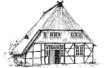
\includegraphics[width=.2\textwidth]{logo-tsh}\\[2ex]
\end{center}
%{\LARGE
%\textbf{6th Workshop Probability and Evolution}}\\[1ex]
%{\Large 
%ay 20 -- May 24, 2024 }\\[2ex]
%bigskip
}
% ===== ===== ===== ===== ===== ===== ===== ===== =====
\setlength{\headsep}{6ex} % Abstand Kopfzeile zu Text
%
\newcommand{\Kopfzeile}{\markboth{\Kopfzeilentext}{~\hfill\Kopfzeilentext\hfill~}}
%
\newcommand{\Kopfzeilentext}{\footnotesize \emph{Dynamics of interacting populations and beyond}}
% https://conferences.cirm-math.fr/3000.html

%\newcommand{\fehlt}[1]{\textcolor{red}{--- --- information is missing --- --- Date:~#1}}
\newcommand{\fehlt}[1]{ \color{red}--- --- information is missing --- ---}
%
\newcommand{\VirtualTalk}{%
\vfill \bggray{~Virtual talks are marked with a gray background.~}}
% ===== ===== ===== =====
\newcommand{\ZAbst}{\rule[-1ex]{0pt}{2ex}\ } % space within title

%\parskip2ex plus.2pt minus1ex

% ==========================================================================
% ==========================================================================
% ==========================================================================
\begin{document}
\sffamily 

\thispagestyle{empty}

{% ---------------------------- Titelseite -----------------------
\begin{center}
\vspace*{1cm}
\addtolength{\textheight}{3.5cm}

{\huge 
\textbf{Dynamics of interacting populations and beyond\\
       at the Theodor-Schwartz-Haus \\[2ex]
 }}
  
\bigskip\bigskip

\textbf{\large September 9 -- September 12, 2025}\\[4ex]
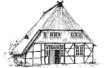
\includegraphics[scale=.4]{logo-tsh}\\[4ex]
\textbf{\large Program and Abstracts}\\[4ex]
Version: \today
\vfill

{Organisation}\\[1.0ex]
Cornelia Pokalyuk \\
Peter Pfaffelhuber\\[2ex]

\bigskip
%{Invited speakers}\\[1.0ex]
%\textcolor{red}{--- list all speakers ??? --- ---}\\[1cm]
% 
{%
\begin{minipage}[c]{.19\textwidth} 
{\bigskip\medskip
\begin{center}%
\fboxsep0pt
%\fbox%
{%\hspace*{2.7ex}

\includegraphics[width=\textwidth, clip
]{Siegel-Uni-Luebeck.svg.png}}\\% Logo
%\fbox
\end{center}}
 \end{minipage}%
 }%
 \hfill
{%
\begin{minipage}[c]{.6\textwidth}
\begin{center}

University of Lübeck\par
Institut for Mathematics
\\[1.25ex]
%  
  University of Freiburg \par  
  Mathematical Institute \par 
  Department of Mathematical Stochastics 
 \end{center}
 \end{minipage}%
 }
\hfill%
%
{\begin{minipage}[c]{.19\textwidth} 
{\bigskip\medskip
\begin{center}%
%\fboxsep0pt\fbox%
{
\includegraphics[width=1.3\textwidth]{UFR-vorlage-designsystem-elemente-uebersicht.png}}
\end{center}}
\end{minipage}
}
\end{center}
}

\pagebreak 
\pagestyle{headings}
\renewcommand{\arraystretch}{1.85}

\Kopf
\vspace*{.75cm}

\textbf{\Large  Monday, May 20, 2024}\medskip

\begin{tabular}{@{}l p{.81\textwidth}@{}}
%\phantom{1}9:30--10:15 &  \textbf{senior xxx} \\
%
9:30--10:15 &  \textbf{Simon Myers}, 
                \sloppy Seeing the forest from the trees: leveraging \mbox{genealogies} to understand evolutionary forces. \\ 
10:15--10:25 &  \textbf{Raphaël Forien},
                Demographic inference for spatially heterogeneous populations using long shared haplotypes. \\ 
10:25--10:35 &  \textbf{Patrick Hoscheit},
                Allele Frequency Spectra for Stationary Branching Processes. \\ 
10:35 & coffee break  \\  
11:00--11:30 &  \textbf{Dave Jacobi}, 
                On/Off super-Brownian motion and its relatives. \\
11:30--12:00 & \textbf{Guillaume Martin}, 
                Epistasis and fitness distributions within and between large asexual populations. \\
%11:30--12:00 &  \textbf{Apolline Louvet}, 
%                Dormancy in urban environments.\\
12:30 & lunch  \\  
16:00--16:45 & \textbf{Jason Schweinsberg}, 
                Speciation induced by dormancy in a model with changing environment.\\ 
16:45--16:55 & \textbf{Jan Lukas Igelbrink}, 
                Ancestral reproductive bias in continuous time branching trees under various sampling schemes.  \\
%16:55--17:05 & \textbf{Yubo Shuai}, 
%                Asymptotics for the site frequency spectrum associated with the genealogy of a birth and death process. \\
%17:05 & coffee break  \\  
16:55--17:25 & \textbf{Nantawat Udomchatpitak}, 
                The Accumulation of Beneficial Mutations and Convergence to a Poisson Process. \\
18:00 & poster session \\
19:30 & dinner 
\end{tabular}

\newpage

\Kopf
\vspace*{.75cm}

\textbf{\Large Tuesday, May 21, 2024}\medskip

\begin{tabular}{@{}l p{.81\textwidth}@{}}
%\phantom{1}9:30--10:15 &  \textbf{senior xxx} \\
%
9:30--10:15 &  \textbf{Sarah Penington}, 
                Gaussian waves in BBM with mean-dependent branching. \\ 
10:15--10:25 & \textbf{Philibert Courau}, 
                The gene's eye-view of quantitative genetics. \\          
10:25--10:35 &  \textbf{Loïc Marrec},
                Evolutionary rescue in a changing environment. \\ 
10:35 & coffee break  \\  
11:00--11:30 &  \textbf{Joao Luiz de Oliveira Madeira}, 
                Functional law of large numbers for a spatial model of the Muller's ratchet. \\
11:30--12:00 &  \textbf{Thomas Hughes}, 
                Interface evolution in bistable spatial models in population genetics: a global approach.\\
12:30 & lunch  \\  
16:00--16:45 & \textbf{Camille Coron}, 
                Condensation in the Kingman house-of-cards model with periodic environment.\\ 
16:45--16:55 & \textbf{Sophie Kersting},
                Testing evolutionary models - Which tree balance index is the most powerful? \\
16:55 & coffee break  \\ 
17:20--17:50 & \textbf{Florin Boenkost}, 
                Dust solutions and the nested Kingman coalescent. \\
17:50--18:35 & \textbf{John Wakeley}, 
                Accounting for pedigrees in models of ancestral genetic processes. \\
18:35--19:30 &  informal online gathering with                     BIRS. \\
19:30 & dinner
\end{tabular}

\newpage

\Kopf
\vspace*{.75cm}

\textbf{\Large Wednesday, May 22, 2024}\medskip

\begin{tabular}{@{}l p{.81\textwidth}@{}}
%\phantom{1}9:30--10:15 &  \textbf{senior xxx} \\
%
9:30--10:15 &  \textbf{Charline Smadi}, 
                Quasi-equilibria and click times for Muller’s ratchet with (binary) tournament selection. \\ 
10:15--10:25 & \textbf{Vianney Brouard}, 
                Genetic composition of supercritical branching populations under power law mutation rates. \\          
10:25--10:35 &  \textbf{Sophia-Marie Mellis},
                Coalescents with Migration in the Moderate Regime. \\ 
10:35 & coffee break  \\  
11:00--11:30 &  \textbf{Zsofia Talyigas}, 
                Different behaviours of the $N$-particle branching random walk. \\
11:30--12:00 &  \textbf{Guillaume Achaz}, 
                Weak genetic draft and the Lewontin’s paradox.\\
12:30 & lunch  \\  
19:30 & dinner
\end{tabular}

\newpage

\Kopf
\vspace*{.75cm}

\textbf{\Large Thursday, May 23, 2024}\medskip

\begin{tabular}{@{}l p{.81\textwidth}@{}}
%\phantom{1}9:30--10:15 &  \textbf{senior xxx} \\
%
9:30--10:15 &  \textbf{Maite Wilke Berenguer}, 
                $\Xi$-coalescents arising from structured populations undergoing bottlenecks. \\ 
10:15--10:25 & \textbf{Carola Sophia Heinzel}, 
                Flat Likelihoods in the Admixture Model. \\          
10:25--10:35 &  \textbf{Raphael Eichhorn},
                On a neutral host-virus model with applications to HCMV. \\ 
10:35 & coffee break  \\  
11:00--11:30 &  \textbf{Bastian Wiederhold}, 
                Interpreting spatial central limit theorems as the asymptotic behavior of two ancestral lineages. \\
11:30--12:00 &  \textbf{Adrian Gonzalez Casanova}, 
                The Seed-Bank Random Graph.\\
12:30 & lunch  \\  
16:00--16:45 & \textbf{Cornelia Pokalyuk}, 
                On the spread of an infection in a host population distributed on $\mathbb{Z}$ with host immunity.\\ 
16:45--16:55 & \textbf{Colin Desmarais}, 
                A branching random walk with noisy selection. \\
16:55--17:05 & \textbf{Berk Perçin},
                Solution of F-KPP Equation Using Chemical Diffusion Master Equation of A Branching Brownian Motion \\
17:05 & coffee break  \\  
17:30--17:40 & \textbf{Maria Gamboa Pérez}, 
                Assessing the feasibility of a re-vaccination program when considering an imperfect vaccine under a Markovian approach. \\
17:40--18:25 & \textbf{Jochen Blath}, 
                Dormancy in population genetics and beyond - recent progress and open challenges. \\
19:30 & dinner
\end{tabular}

\newpage

\Kopf
\vspace*{.75cm}

\textbf{\Large Friday, May 24, 2024}\medskip

\begin{tabular}{@{}l p{.81\textwidth}@{}}
%\phantom{1}9:30--10:15 &  \textbf{senior xxx} \\
%
9:30--10:15 &  \textbf{Félix Foutel-Rodier}, 
                Emergence of multiple mergers in structured populations and semi-pushed fronts. \\ 
10:15--10:25 & \textbf{Mathilde André}, 
                Genealogies in multitype frequency-dependent branching processes via spinal decomposition. \\          
10:25--10:35 &  \textbf{Florence Bansept},
                How does intermittent feeding shape the gut microbiome? \\ 
10:35 & coffee break  \\  
11:00--11:30 &  \textbf{Anna Kraut}, 
                A multi-scale model for DNA methylation. \\
11:30--12:00 &  \textbf{Manuel Esser}, 
                Fitness valleys and multi-scale analysis in changing environment.\\
12:30 & lunch  \\  

\end{tabular}

\newpage





%\VirtualTalk


\newpage

% % \Impressum  % nur für Programm-Seiten aktivieren

%\pagebreak~\pagebreak


% ------------------ Abstracts -----------


\setlength{\topmargin}{1cm}
\addtolength{\textheight}{-2cm}
\pagestyle{myheadings}
\Kopfzeile % Definition Kopfzeile

\section*{\sffamily Abstracts}
\subsection*{\sffamily Monday, May 20, 2024}
\bigskip\bigskip

\noindent
{\Large Seeing the forest from the trees:\ZAbst leveraging genealogies to understand evolutionary forces}\\[1ex]
{\large 
\textbf{Simon Myers}\\[1ex] University of Oxford}\\[2ex]
Genetic differences are a critical driver of disease risk and healthy variation, across the tree of life. Mutations arise and spread in our distant, genealogical ancestors, and so genetic variation data can provide a window into our evolutionary past, allowing us to understand processes such as population size changes, admixture, natural selection, and even evolution of the mutation and recombination processes that generate the variation itself. It has long been recognised that knowledge of genealogical relationships among individuals would allow us to capture almost all the information available from such data. However, only in recent years has it become computationally feasible to infer such genealogies, genome-wide, from variation patterns. One such method, Relate, developed in our lab, allows approximate inference of genealogical trees under coalescent-like models, for up to tens of thousands of samples. Here, we will show that a powerful approach for inference is to identify and characterise departures from the relatively simple models used to build these trees. By defining a "population" as a set of coalescence rates between labelled individuals backwards in time, we can uncover variability in these rates, and use a single collection of trees to identify ancient mixing events among populations -- including "ghost" groups we have never sampled -- natural selection favouring the descendents of particular branches of the genealogy, and departures from mathematical expectations under clock-like behaviour, indicating disruption of recombination or mutation.

\bigskip \bigskip 
%----------------------------------------------%

\noindent
{\Large \sloppy Demographic \ZAbst inference for spatially heterogeneous populations using long shared haplotypes}\\[1ex]
{\large 
\textbf{Raphaël Forien}\\[1ex] INRAE Avignon}\\
%\url{raphael.forien@inrae.fr}\\
[2ex]
We introduce a variant of the spatial Lambda-Fleming–Viot process to model a population occupying a continuous spatial habitat with a sharp discontinuity of the dispersal rate and effective population density at some interface. We then develop a method to infer the strength of dispersal and the effective population density in both regions using the length distribution of haplotype segments shared by individuals sampled from the population at different locations. The method combines a composite likelihood approach with an analytical formula for the expected number of shared haplotype segments, which involves the transition density of a skew diffusion arising as a scaling limit of the trajectories of ancestral lineages. We then demonstrate the efficiency of this method on a range of simulated data sets.
\\
This is joint work with Harald Ringbauer and Graham Coop.

\bigskip \bigskip  %----------------------------------------------%

\noindent
{\Large Allele\ZAbst Frequency Spectra for Stationary Branching \\ Processes}\\[1ex]
{\large 
\textbf{Patrick Hoscheit}\\[1ex] INRAE, France}\\[2ex]
%\url{patrick.hoscheit@inrae.fr}\\
The allele frequency spectrum (AFS) describes the genetic diversity of a sample from a given population; it can be used to infer ancestral population size, assess the presence of selection or latent structure in the population. In this talk, I will show how these statistics can be computed for continuous state branching processes (CSBP) in the stationary case, when the processes are conditioned not to go extinct. These computations rely on a representation of the genealogy of a sample uniformly chosen in the extant population at a fixed time. I will also show how to describe the frequency spectrum in the limit of a large sample, following results on coalescent point processes by Duchamps and Lambert (2018). Joint work with Romain Abraham and Jean-François Delmas. 

\bigskip \bigskip  %----------------------------------------------%

\noindent
{\Large On/Off super-Brownian motion and its relatives}\\[1ex]
{\large 
\textbf{Dave Jacobi}\\[1ex] TU Berlin}\\[2ex]
%\url{jacobi@math.tu-berlin.de}\\
On/Off super-Brownian motion is a super-Brownian motion with an additional Dormancy mechanism. It arises as a large population limit of a binary branching Brownian motion with Dormancy. This novel process has many interesting properties that are often closely related to classical super-Brownian motion, but at the same time exhibit new and different behaviour. For example, considering the dynamics of the total active mass and the total dormant mass, we discover that its long term behaviour strongly differs from the long term behaviour of the classical process: On/off super-Brownian motion does not die out in finite time, whereas classical super-Brownian motion does. However, the total active mass of on/off super-Brownian motion does die out in finite time with positive probability.
\\
If time permits, we will furthermore look at the corresponding Stochastic Partial Differential Equation, that governs the evolution of the measure-valued processes density. This SPDE looks surprisingly different from what one might expect, hinting at an implicit non-local branching behaviour. We will also show how one could couple the on/off superprocess with its classical version using an on/off Brownian snake. Adding Dormancy to a Brownian snake essentially breaks the Markov property of the underlying excursion and pushes the excursion to infinite heights. As an application, the on/off snake will make it possible to also couple the ranges of the on/off super-Brownian motion and its classical counterpart, which, despite the intuitive nature of the statement, turns out to be technically challenging.
This research is based on ongoing joint work with Jochen Blath, Matthew Buckland and Matthias Winkel. 
\\\url{https://arxiv.org/abs/2307.10968}

\bigskip \bigskip  %----------------------------------------------%

%\bigskip \bigskip  %----------------------------------------------%

\noindent
{\Large Epistasis\ZAbst and fitness distributions within and between large asexual populations}\\[1ex]
{\large 
\textbf{Guillaume Martin}\\[1ex] CNRS, ISEM UMR 5554, France}\\[2ex]
%\url{guillaume.martin@umontpellier.fr}\\
I consider the dynamics of the fitness distribution in large asexual populations climbing a single fitness peak in a phenotype-fitness landscape. The effects of selection, mutation (epistatic-infinite types model)  and genetic drift are described in terms of a (rescaled) PDE satisfied by the Laplace transform of the fitness distribution (Kolmogorov forward equation). Approximate solutions for weak or strong selection provide explicit trajectories of expected  fitness moments in large populations.  The variation and bias  introduced by finite (large) populations will be explored approximately by comparing the infinite population solution with an approximate solution to the finite population Kolmogorov equation. Comparisons to fitness trajectories in Lenski's long term evolution experiment will serve to illustrate the method. The joint distribution of genetic distance to the ancestor and fitness will be tackled if time allows. 

%\noindent
%{\Large Dormancy in urban environments}\\[1ex]
%{\large 
%\textbf{Apolline Louvet}\\[1ex] TU Munich}\\[2ex]
%%\url{apolline.louvet@polytechnique.edu}\\
%Understanding the drivers of biodiversity in urban environments is an important question in urban ecology. As urban environments are very fragmented and subject to frequent disruptions, the biological traits associated to a higher survival probability are expected to differ from the ones selectively advantaged in more natural environments. 
%\\
%The goal of this contribution is to investigate this question through the lens of dormancy. To do so, we introduce a stochastic process for plant dynamics in urban environments. We show the existence of a critical local extinction probability above which a seed bank is needed to ensure survival. Then, we make use of the theoretical results obtained to construct a "metric" of the extinction risk at the metapopulation scale. We apply our framework to a dataset of floristic inventories carried out in 1300 tree bases in Paris, France, allowing us to identify several biological traits associated to higher survival probabilities in urban tree bases. 
%Based on a joint work with Nathalie Machon (CESCO, MNHN) and Clément Mantoux. 
%\\
%url{https://arxiv.org/abs/2107.13359}


\bigskip
\bigskip

%----------------------------------------------%

{\Large  
Speciation\ZAbst induced by dormancy in a model with changing environment}\\[1ex]
{\large 
\textbf{Jason Schweinsberg}\\[1ex] University of Calofornia, San Diego}\\[2ex]
We consider a population model in which the season alternates between winter and summer, and individuals can acquire mutations either that are advantageous in the summer and disadvantageous in the winter, or vice versa.  Also, we assume that individuals in the population can either be active or dormant, and that individuals can move between these two states.  Dormant individuals do not reproduce but do not experience selective pressures.  We show that, under certain conditions, over time we see two waves of adaptation.  Some individuals repeatedly acquire mutations that are beneficial in the summer, while others repeatedly acquire mutations that are beneficial in the winter.   Individuals can survive the season during which they are less fit by entering a dormant state.  This result suggests that, for populations in fluctuating environments, dormancy may have the potential to induce speciation.  This is joint work with Fernando Cordero and Adrian Gonzalez Casanova.

\bigskip \bigskip  %----------------------------------------------%

\noindent
{\Large Ancestral\ZAbst reproductive bias in continuous time branching trees under various sampling schemes}\\[1ex]
{\large 
\textbf{Jan Lukas Igelbrink}\\[1ex] GU Frankfurt \& JGU Mainz}\\[2ex]
%\url{igelbrin@math.uni-frankfurt.de}\\
Cheek and Johnston (Journal of Mathematical Biology, 2023) consider a continuous-time Bienaymé-Galton-Watson tree conditioned on being alive at time $T$. They study the reproduction events along the ancestral lineage of an individual randomly sampled from all those alive at time $T$. We give a short proof of an extension of their main results to the more general case of Bellman-Harris processes. Our proof also sheds light onto the probabilistic structure of the rate of the reproduction events. A similar method will be applied to explain (i) the different ancestral reproduction bias appearing in work by Geiger (Journal of Applied Probability, 1999) and (ii) the fact that the sampling rule considered by Chauvin, Rouault and Wakolbinger (Stochastic Processes and their Applications, 1991) leads to a time homogeneous process along the ancestral lineage.
\\\url{https://arxiv.org/abs/2309.05998}


%\bigskip \bigskip  %----------------------------------------------%

%\noindent
%{\Large Asymptotics\ZAbst for the site frequency spectrum associated with the genealogy of a birth and death process}\\[1ex]
%{\large 
%\textbf{Yubo Shuai}\\[1ex] University of California, San Diego}\\[2ex]
%\url{yushuai@ucsd.edu}\\
%Consider a birth and death process started from one individual in which each individual gives birth at rate $\lambda$ and dies at rate $\mu$, so that the population size grows at rate $r = \lambda - \mu$.  Lambert, and Harris, Johnston, and Roberts came up with methods for constructing the exact genealogy of a sample of size $n$ taken from this population at time $T$.  We use the construction of Lambert, which is based on the coalescent point process, to obtain asymptotic results for the site frequency spectrum associated with this sample. In the supercritical case $r > 0$, our results extend the results of Durrett for exponentially growing populations. In the critical case $r = 0$, our results parallel those that Dahmer and Kersting obtained for Kingman's coalescent. 


\bigskip \bigskip  %----------------------------------------------%
%\newpage

\noindent
{\Large The\ZAbst Accumulation of Beneficial Mutations and Convergence to a Poisson Process}\\[1ex]
{\large 
\textbf{Nantawat Udomchatpitak}\\[1ex] Mahidol University, Thailand}\\[2ex]
%\url{nantawat.udo@mahidol.ac.th}\\
We consider a model of a population with fixed size $N$, which is subjected to an unlimited supply of beneficial mutations at a constant rate $u_N$. Individuals with $k$ beneficial mutations have the fitness $(1+s_N)^k$. Each individual dies at rate 1 and is replaced by a random individual chosen with probability proposition to its fitness. In this work, we show that when $u_N \ll 1/(N \log N )$ and $s_N \sim 1/N^{1-d}$ where $0<d<1$, large numbers of beneficial mutations are always present in the population at the same time, competing against each other, yet the fixation times of beneficial mutations after a time scaling converge to the times of a Poisson process. This is joint work with Jason Schweinsberg. 

\subsection*{Poster session}
See page \pageref{ss:poster}.

\newpage 
\subsection*{\sffamily Tuesday, May 21, 2024}

%----------------------------------------------%
{\Large  
Gaussian waves in BBM with mean-dependent branching}\\[1ex]
{\large 
\textbf{Sarah Penington}\\[1ex] University of Bath}\\[2ex]
We consider a continuous-space analogue of a population model introduced by Yu, Etheridge and Cuthbertson. We prove a hydrodynamic limit result that allows us to show that for a large total population size, at large times the empirical distribution of the particle positions evolves approximately according to an accelerating Gaussian wave. 
Based on joint work with Erin Beckman.



\bigskip \bigskip  %----------------------------------------------%

\noindent
{\Large The gene's eye-view of quantitative genetics}\\[1ex]
{\large 
\textbf{Philibert Courau}\\[1ex] IBENS/CIRM Collège-de-France/ University of Vienna}\\[2ex]
%\url{philibert.courau@gmail.com}\\
Modelling the evolution of a continuous trait in a biological population is one of the oldest problems in evolutionary biology, which led to the birth of quantitative genetics. With the recent development of GWAS methods, it has become essential to link the evolution of the trait distribution to the underlying evolution of allelic frequencies at many loci, co-contributing to the trait value. The way most articles go about this is to make assumptions on the trait distribution, and use Wright's powerful formula to model how the evolution of the trait translates on each individual locus. Here, we take a gene's eye-view of the system, starting from an explicit finite-population-size finite-loci model with selection, drift, recombination and mutation, in which the trait value is a direct product of the genome. First, we let the recombination rate go to infinity and prove that we reach linkage equilibrium. Then, we let the number of loci go to infinity under the assumption of no linkage, and characterize the limit behavior of a given locus with a McKean-Vlasov SDE and the corresponding Fokker-Planck PDE. This yields powerful results, including independence of two loci, explicit stationary distribution for allelic frequencies at a given locus (under some hypotheses on the fitness function), and normality of the trait distribution. We recover Wright's formula and the breeder's equation as special results.



\bigskip
\bigskip

%----------------------------------------------%

{\Large  
Evolutionary rescue in a changing environment}\\[1ex]
{\large 
\textbf{Loïc Marrec}\\[1ex] Institute for Ecology and Evolution -- Universität Bern}\\[2ex]

No environment is constant over time, and environmental fluctuations impact the outcome of evolutionary dynamics. Survival of a population not adapted to some environmental conditions is threatened unless, for example, a mutation rescues it, an eco-evolutionary process termed evolutionary rescue.  We investigated evolutionary rescue in an environment that fluctuates
between a favorable state, in which the population grows, and a harsh state, in which the population declines. We developed a stochastic model that includes both population dynamics and genetics. We derived analytical predictions for the mean extinction time of a non-adapted population given that it is not rescued, the probability of rescue by a mutation, and the mean appearance time of a rescue mutant, which we validated using numerical simulations. We found that stochastic environmental fluctuations, resulting in quasi-periodic environmental changes, accelerate extinction and hinder evolutionary rescue compared with deterministic environmental fluctuations, resulting in periodic environmental changes. We demonstrated that high equilibrium population sizes and per capita growth rates maximize the chances of evolutionary rescue. Finally, we showed that an imperfectly harsh environment, which does not fully prevent births but makes the death rate to birth rate ratio much greater than unity, has almost the same rescue probability as a perfectly harsh environment, which fully prevents births. Our results apply to antimicrobial resistance and conservation biology. 


\bigskip \bigskip  %----------------------------------------------%

\noindent
{\Large Functional\ZAbst law of large numbers for a spatial model of the Muller's ratchet}\\[1ex]
{\large 
\textbf{Joao Luiz de Oliveira  Madeira}\\[1ex] University of Bath, UK}\\[2ex]
%\url{jldom20@bath.ac.uk}\\
In this work, we study the deterministic scaling limit of a model introduced by Foutel-Rodier and Etheridge in 2020 to study the impact of cooperation and competition on the fitness of an expanding asexual population whose individual birth and death rates depend on the local population density. The interacting particle system can be mathematically described as particles performing symmetric random walks that undergo a birth-death process with rates that depend on the local number of particles. Phenomenologically, each particle represents a chromosome, and we keep track during the process of two features of each particle: its location and its number of deleterious mutations.  After each birth event, with some positive probability, the daughter particle can acquire an additional mutation which will decrease its reproduction rate when compared to its parent. We show that under an appropriate scaling, the process converges weakly to a countable system of partial differential equations, proving a conjecture of Foutel-Rodier and Etheridge. For the case where the reaction term satisfies an FKPP condition, we prove a conjecture of Foutel-Rodier and Etheridge regarding the spreading speed of the population into an empty habitat. We also prove some further results regarding the asymptotic behaviour of the system of PDEs in the monostable case. This is a joint work with Marcel Ortgiese and Sarah Penington. 


\bigskip \bigskip  %----------------------------------------------%

\noindent
{\Large Interface\ZAbst evolution in bistable spatial models in population genetics: a global approach}\\[1ex]
{\large 
\textbf{Thomas Hughes} \\[1ex] University of Bath}\\[2ex]
%\url{th2275@bath.ac.uk}\\
We consider spatial stochastic population models exhibiting bistability. In such models, narrow interfaces tend to form between regions dominated by one of the two stable states. To understand how the population evolves, we may study the dynamics of these interfaces in time. For several bistable population models, it is known from recent work that the limiting interface, under certain rescalings, evolves by a geometric evolution called mean curvature flow. This interface evolution is known to develop singularities in finite time, which imposes a short-time constraint and regularity assumptions on the convergence results.
\\
In this talk, I will first discuss some models exhibiting this phenomenon, including a variant of the Spatial Lambda Fleming-Viot model with selection against heterozygosity, and results concerning their interfaces. I will then discuss an ongoing work which uses tools from analysis, in particular level-set methods and the theory of viscosity solutions, to improve upon recent interface convergence results for a broad class of bistable population models. In particular, we show that the interfaces converge globally in time to a generalized mean curvature flow. 
\\
This is joint work with Jessica Lin (McGill). 


\bigskip \bigskip
%----------------------------------------------%

{\Large  
Condensation\ZAbst in the Kingman house-of-cards model with periodic environment}\\[1ex]
{\large 
 \textbf{Camille Coron}\\[1ex] Université Paris-Saclay}\\[2ex]

Kingman's house-of-cards model aims at studying the impact of mutation and selection on individuals fitness distribution dynamics. The dynamics is defined through the recursive equation : $$p_{n+1}(dx)=\beta_n q_n(dx) + (1-\beta_n)\frac{x p_n(dx)}{\int x p_n(dx)},$$ where the environment $(\beta_n,q_n)$ gives the mutation probability and mutant fitness distribution at time $n$. With Olivier Hénard (Laboratoire de Mathématiques d'Orsay) we study a version of this modele for which environment is periodic. We prove the convergence of this dynamics and give an explicit criterion on parameters, under which a condensation phenomenon at optimal fitness appears.

\bigskip \bigskip  %-----------------------------------------%
\newpage 
\noindent
{\Large Testing\ZAbst evolutionary models - Which tree balance index is the most powerful?}\\[1ex]
{\large 
\textbf{Sophie Kersting}\\[1ex] University of Greifswald, Germany}\\[2ex]
%\url{sophie.kersting@uni-greifswald.de}\\
Tree shape statistics, particularly measures of tree (im)balance, play an important role in the analysis of the topology of phylogenetic trees. With applications ranging from testing evolutionary models to studying the impact of fertility inheritance and selection, or tumor development and language evolution, the assessment of tree balance is crucial. Currently, a multitude of balance indices, at least 30, can be found in the literature, alongside numerous other tree shape statistics.
\\
This diversity prompts essential questions: How can we minimize the selection of indices to mitigate the challenges of multiple testing? Is there a preeminent balance index tailored to specific tasks? Previous studies comparing the statistical power of indices in detecting trees deviating from the Yule model have been limited in scope, utilizing only a subset of indices and alternative tree models.
\\
This research expands upon the examination of index power, encompassing all established indices and a broader array of alternative models. Our investigation reveals distinct groups of balance indices better suited for different alternative tree models, suggesting that decisions on balance index selection can be enhanced with prior knowledge. Furthermore, we present an {\tt R} software package which allows the inclusion of new indices and models, thus facilitating future research. This software package enables researchers to efficiently compare and assess the viability even of newly developed indices for specific tasks. Additionally, it assists in determining which existing index is most suitable for detecting trees constructed under any alternative tree model given any null model. 




\bigskip \bigskip  %----------------------------------------------%

\noindent
{\Large Dust solutions and the nested Kingman coalescent}\\[1ex]
{\large 
\textbf{Florin Boenkost}\\[1ex] University of Vienna}\\[2ex]
%\url{florin.boenkost@univie.ac.at}\\
The nested Kingman Coalescent $(\mathcal{K}^n_t, t\geq 0)$ describes the genealogy of a population which experienced speciation events forward in time. This can be envisioned as trees within a tree. The species tree (the outer tree) is assumed to be a $n$-Kingman coalescent. Additionally, each pair of gene lineages is able to coalesce at rate $1$, given they belong to the same species. Initially, we assume that there are $\ell_n \ll n$ lineages per species.
\\
Here, we focus on the empirical measure $g^n_{t}= \frac{1}{s^n_t} \sum_{i=1}^{s_t^n} \delta_{\Pi_t^n (i)}$ of block sizes in the nested coalescent, where $\Pi_t^n (i)$ denotes the number of gene lineages in  species $i$. As the number of species tends to infinity we show convergence towards a solution $u(t,x)$ of the Smoluchowski coagulation-transport equation
\begin{align*}
	\partial_t u = \partial_x \left( \frac{x^2}{2} u\right) + \frac{1}{t} ( u \star u -u ),
\end{align*}
where $u \star u$ denotes the convolution. In particular, if there are fewer lineages per species than species itself, $g_t^n$ converges to a \emph{dust solution} $u(t,x)$, meaning that $u(t,x) \to \delta_0(dx)$ as $t\to 0$. Dust solutions of this equation appeared in the work of [Lambert and Schertzer, 2019] and a priori there are infinitely many. We show that the solution is unique up to a scaling parameter which encodes the initial number of lineages per species. This is accomplished through a probabilistic representation of the PDE, which in turn can be extended to provide a stochastic representation of all dust solutions in terms of a martingale. Lastly, we give an outlook on how these results can be used to get access to the site frequency spectrum of the nested Kingman coalescent.
\\
This talk is based on joint work with Emmanuel Schertzer. 

\bigskip
\bigskip

%----------------------------------------------%

\enlargethispage{1cm}
{\Large  
Accounting\ZAbst for pedigrees in models of ancestral genetic processes}\\[1ex]
{\large 
\textbf{John Wakeley}\\[1ex] University of Harvard}\\[2ex]
The genealogy, or pedigree, of a diploid population is an object fixed by past events. Gene genealogies across the entire genome are the results of genetic transmission through the single pedigree. In this work, the distribution of the time to the common ancestor of a sample of size two at an autosomal locus, conditional on the pedigree, is analyzed in the limit as the population size tends to infinity. This gives a prediction for the distribution of coalescence times among unlinked loci conditional on their shared pedigree. If the pedigree was produced by Wright-Fisher reproduction, the limiting distribution of coalescence times is the same as under the standard neutral, Kingman coalescent. In this case predictions about genetic variation do not depend on the pedigree. But if very large reproductive outcomes ({\em big families}) are interspersed in the pedigree, the limiting ancestral process is a standard-neutral or Kingman coalescent punctuated by big-family events in which bursts of coalescence occur. In this case predictions about genetic variation do depend on the pedigree. This implies a new sort of model in coalescent theory, as the multiple-merger coalescent models so-far developed for similar scenarios do not account for the pedigree. Instead they implicitly average over the pedigree. Additional results are illustrated using simulations, and their implications for inference and understanding multi-locus data are discussed. 

This talk will also include an introduction for CIRM participants to the new Society for Modeling and Theory in Population Biology (\url{smtpb.org}) which has its first in-person meeting during the same week (May 20-24) at the Banff International Research Station in Canada. It will be followed by an informal online gathering between participants at CIRM and BIRS.  

\newpage
\subsection*{\sffamily Wednesday, May 22, 2024}

%----------------------------------------------%

\noindent
{\Large 
Quasi-equilibria\ZAbst and click times for Muller’s ratchet with (binary) tournament selection}\\[1ex]
{\large\textbf{Charline Smadi}\\[1ex] LESSEM, Inrae and Institut Fourier, Grenoble}\\[2ex]
%\\[1ex] {\em Format:} Talk 10 minutes; 
%\\ Poster possible: Yes
Consider a population of $N$ individuals, each of them carrying a type in $\N_0$. The population evolves according to a Moran dynamics with selection and mutation, where an individual of type $k$ has the same selective advantage over all individuals with type $k′ > k$, and type $k$ mutates to type $k + 1$ at a constant rate. This model is a variation of the classical Muller’s ratchet: there the selective advantage is proportional to $k′ − k$.  
\\
I will describe how, for a regime of selection strength and mutation rates which is between the regimes of weak and strong selection/mutation, we obtain the asymptotic rate of the click times of the ratchet, and reveal the quasi-stationary type frequency profile between clicks. The large population limit of this profile is characterized as the normalized attractor of a {\em dual} hierarchical multitype logistic system. An important role in the proofs is played by a graphical representation of the model, both forward and backward in time, and a central tool is the ancestral selection graph decorated by mutations.
\\
In a work of Etheridge  et al. [EPW09], the authors obtained approximations of the classical ratchet, allowing to identify a crucial parameter for the speed of accumulation of deleterious mutations. One of their approximations for the dynamics of the best class, after a parameter change, correspond exactly to the dynamics of the best class in the tournament racthet. We will discuss how this could help us studying the classical ratchet.
\\
[EPW09] A. M. Etheridge, P. Pfaffelhuber, and A. Wakolbinger. How often does the ratchet click? Facts, heuristics, asymptotics, page 365–390. London Mathematical Society Lecture Note Series. Cambridge University Press, 2009.
\\
This is a joint and ungoing work with A. Gonzalez Casanova, J. Lukas Igelbrink and A. Wakolbinger


\bigskip \bigskip  %----------------------------------------------%

\noindent
{\Large Genetic\ZAbst composition of supercritical branching populations under power law mutation rates}\\[1ex]
{\large\textbf{ Vianney  Brouard}\\[1ex] ENS de Lyon}\\[2ex]
%\\[1ex] {\em Format:} Talk 10 minutes; 
%\\ Poster possible: Yes
We aim at understanding the evolution of the genetic composition of cancer cell populations. To this aim, we consider a branching individual based model representing a cell population where cells divide, die and mutate along the edges of a finite directed graph $(V,E)$. The process starts with only one cell of trait~0. Following typical parameter values in cancer cell populations we study the model under large population and power law mutation rates limit, in the sense that the mutation probabilities are parameterized by negative powers of $n$ and the typical sizes of the population of our interest are positive powers of $n$. Under non-increasing growth rate condition (namely the growth rate of any sub-population is smaller than the growth rate of trait~0), we describe the time evolution of the first-order asymptotics of the size of each sub-population on the $\log n$ time scale, as well as in the random time scale at which the initial population, resp. the total population, reaches the size $nt$. In particular, such results allow to characterize whose mutational paths along the edges of the graph are actually contributing to the size order of the sub-populations. Without any condition on the growth rate, we describe the time evolution of the orders of magnitude of each sub-population. Adapting techniques from Durrett and Mayberry (2011), we show that these converges to positive deterministic non-decreasing piecewise linear continuous functions, whose slopes are given by an algorithm. \\
\url{https://arxiv.org/abs/2309.12055}

%% \noindent
%% {\em Decision: }
%% T1S

\bigskip \bigskip  %----------------------------------------------%

\noindent
{\Large Coalescents with Migration in the Moderate Regime}\\[1ex]
{\large 
\textbf{Sophia-Marie Mellis}\\[1ex] Bielefeld University, Germany}\\[2ex]
%\url{smellis@math.uni-bielefeld.de}\\ 
Multi-type models have recently experienced renewed interest in the stochastic modeling of evolution. This is partially due to their mathematical analysis often being more challenging than their single-type counterparts; even in classical settings of population genetics, our understanding is still incomplete. An example of this is the multi-type Moran model with moderate mutation.
\\
In this talk, we consider a multi-type coalescent starting with $K^{\gamma}$ colored singletons ($\gamma \geq 1$) with $d \geq 2$ possible colors. The process is described by a continuous-time Markov chain with values on the colored partitions of the colored integers in $\{1, \ldots, K^{\gamma}\}$; blocks of the same color coalesce at rate $1$, while they are also allowed to change color (mutation/migration) at a rate proportional to $K$. This coalescent can be interpreted as a prototype model to describe the genealogy of a multi-type Moran model with moderate mutation.
\\
Given this setting, we study the asymptotic behavior, as $K\to\infty$ at small times, of the vector of empirical measures, whose $i$-th component keeps track of the blocks of color $i$ at time $t$ and the initial coloring of the integers composing each of these blocks. We show that, in the proper time-space scaling, it converges to a multi-type branching process (case $\gamma = 1$) or a multi-type Feller diffusion (case $\gamma > 1$). If time permits, we will also show an application of this result to the site-frequency-spectrum.
\\
This is joint work with Fernando Cordero, Sebastian Hummel and Emmanuel Schertzer. 

\bigskip \bigskip  %----------------------------------------------%

\noindent
{\Large Different\ZAbst behaviours of the $N$-particle branching random walk}\\[1ex]
{\large 
\textbf{Zsofia Talyigas}\\[1ex] University of Vienna}\\[2ex]
%\url{zsofia.talyigas@univie.ac.at}\\
The $N$-particle branching random walk is a discrete time branching particle system with selection. We have $N$ particles located on the real line at all times. At every time step each particle is replaced by two offspring, and each offspring particle makes a jump of non-negative size from its parent's location, independently from the other jumps, according to a given jump distribution. Then only the $N$ rightmost particles survive; the other particles are removed from the system to keep the population size constant.
\\
This process shows very different behaviours with different jump distributions in terms of speed and genealogy. The speed in the ‘light-tailed’ case (when the jump distribution has some exponential moments) was studied by B\'erard and Gou\'er\'e, and the polynomial-tailed case was investigated in the work of B\'erard and Maillard. As these two cases are significantly different from each other, we aimed to fill the gap with our result on the intermediate stretched exponential case. We describe the first order and give lower and upper bounds on the second order of the asymptotic speed as the number of particles $N$ goes to infinity. If time allows I will also discuss our genealogy result in the polynomial case, which says that at a typical large time the genealogy of the population is given by a star-shaped coalescent.
\\
This is joint work with Sarah Penington and Matthew Roberts. 

\bigskip \bigskip  %----------------------------------------------%

\noindent
{\Large Weak genetic draft and the Lewontin’s paradox}\\[1ex]
{\large 
\textbf{Guillaume Achaz}\\[1ex] Université Paris-Cité, Collège de France}\\[2ex]
%\url{guillaume.achaz@college-de-france.fr}\\
Neutral theory assumes that in a population of size $N$, diversity results from an equilibrium between new mutations arising at rate $\mu$ and genetic drift that purge them at rate $1/N$, predicting an equilibrium value proportional to $N\mu$. The difference between this expectation and the much lower observed molecular diversity is known as the Lewontin’s paradox of variation. Here, we investigate the effect of genetic draft, a regime of evolution where recurrent sparse selective sweeps entirely drive the diversity of surrounding loci. More specifically, we focus on the neglected distant effect of selective sweeps on remote neutral loci, where the effect of a single sweep is almost negligible. We derived novel mathematical approximations of this underexplored regime and show that under weak genetic draft, diversity at neutral loci is a power law of the population size: $N_e = K_A \cdot N^{2A}$, for $A < 0.5$, where $A$ is the ratio between recombination rate and coefficient of selection ($A = c/s$). Interestingly the Site Frequency Spectrum at neutral loci is identical to the one produced by genetic drift, as the underlying coalescent tree is an $n$-Kingman coalescent. In brief, weak genetic draft produces patterns of diversity that look entirely neutral, while being drastically reduced in magnitude. Ultimately, our study points to the need to explore evolutionary models for which diversity looks neutral but does not scale linearly with population size. 
\\ {\em URL:} \url{https://www.biorxiv.org/content/10.1101/2023.07.19.549703v3}

\newpage

\subsection*{\sffamily Thursday, May 23, 2024}

{\Large $\Xi$-coalescents\ZAbst arising from structured populations undergoing bottlenecks}\\[1ex]
{\large 
\textbf{Maite Wilke Berenguer}\\[1ex] HU Berlin}\\[2ex]
We consider demographic bottlenecks, i.e. severe declines in population size that can last many generations, in a spatially structured population. This is motivated by the cycles of overfishing and fishing moratoria in different regions that Atlantic Cod has undergone as a commercially relevant fish. We build an individual based model and distiguish between two kinds of bottlenecks ({\em soft}, if the size of the population during the bottleneck is of smaller order than the total population size, but tends to infinity, "drastic", if the size of the population during the bottleneck remains bounded as the total population size tends to infinity) following ideas from (Gonzalez Casanova, Miro Pina \& Siri-Jegousse, 2022). In both cases we study the effect on the allele frequency process and its genealogical dual, a multi-type $\Xi$-coalescent featuring simultaneous multiple mergers and migrations.
This talk is based on ongoing joint work with A. Etheridge, J.Koskela, M. Dai Pra.
\bigskip \bigskip  %----------------------------------------------%

\enlargethispage{1cm}
\noindent
{\Large Flat Likelihoods in the Admixture Model}\\[1ex]
{\large 
\textbf{Carola Sophia Heinzel}\\[1ex] University of Freiburg}\\[2ex]
%\url{carola.heinzel@stochastik.uni-freiburg.de}\\
In the admixture model it is a common aim to estimate the allele frequencies and the individual’s ancestries (IA) from genotype data. Frequently used softwares implementing this model, such as {\sc ADMIXTURE} or {\sc STRUCTURE}, employ a maximum likelihood approach. However, the maximum of the likelihood is usually not unique. This non-uniqueness might result in a large set of values of the IA and the allele frequencies with the same likelihood as the maximum likelihood estimator (MLE). To asses whether the maximum likelihood approach is feasible, it is important to know every MLE. The previous approach for inferring the MLEs is to run ADMIXTURE several times. Consequently, many MLEs might remain unknown.  
\\
We developed an algorithm (and for simple cases an analytic solution) that gives nearly every MLE for the given data, if one MLE is known. We used these results to name characteristics of the markers and the individuals that prevent large differences between the MLEs. Furthermore, we identified conditions that imply a unique MLE and we proved under weak constraints the consistency of the MLE for the IA to the true IA. We applied our method for inferring the MLEs to data from the 1000 Genomes Project, i.e.\ we answer for this data the question whether the differences between the MLEs are large. 
\\
This talk is based on joint work with Peter Pfaffelhuber.

\bigskip \bigskip  %----------------------------------------------%

\noindent
{\Large On a neutral host-virus model with applications to HCMV}\\[1ex]
{\large 
\textbf{Raphael Eichhorn}\\[1ex] Goethe Universität Frankfurt}\\[2ex]
%\url{eichhorn@math.uni-frankfurt.de}\\
Some viruses including the widespread Human Cytomegalovirus (HCMV) are able to maintain a high level of genetic diversity within hosts and across the whole virus population even in relatively conserved genomic regions. However, if we model the frequencies of two competing virus types in a single host using an ordinary Moran model with rare mutations we would expect a decrease of diversity over time, eventually leading to the extinction of one virus type. Thus, this approach is too simplistic: real viral populations may be influenced by not only viral reproduction and mutation but also other evolutionary forces including but not limited to host birth and death, recombination and interactions between hosts leading to reinfections. Previous research by Pokalyuk and Wakolbinger investigated such a model considering a single locus and assuming that viral reproduction within hosts is driven by balancing selection. They showed how under these forces a high level of genetic diversity can be maintained over time. We extend this model to finitely many loci, add recombination between loci, but assume neutral viral reproduction within hosts. We analyze in which parameter regime non-trivial within host viral diversity can be observed under rare mutation but with standing genetic variation and determine the asymptotic within host type frequency distribution. Based on these findings we fit our model to actual observed genotype frequencies from Austrian HCMV patients. We find that the neutral model describes the data surprisingly well. 

\bigskip \bigskip  %----------------------------------------------%

\noindent
{\Large Interpreting\ZAbst spatial central limit theorems as the asymptotic behavior of two ancestral lineages}\\[1ex]
{\large 
\textbf{Bastian Wiederhold}\\[1ex] University of Oxford}\\[2ex]
%\url{bastian.wiederhold@stats.ox.ac.uk}\\
Based on two projects joint with Raphael Forien, I would illustrate the strengths of a novel approach to interpret central limit theorems of spatial population processes in terms of the probability of identity by descent, which reflects the asymptotic behavior of two ancestral lineages. This technique has recently been introduced by Raphael (1). 
\\
In the first project (2), we study asymptotically Brownian or stable ancestral lineages. The resulting central limit theorems in (1) could be interpreted as coalescence happening locally in the Brownian and non-locally in the stable case. Here, we decorrelate the coalescence and motion behavior showing that each motion can appear with a variety of coalescence kernels. Surprisingly, we show that stable lineages with only local coalescence and even Brownian lineages with non-local coalescence are possible.
\\
In the second project (preprint upcoming), we study a spatial population with varying population size. The varying population density renders the dual process non-Markovian making a backwards-in-time approach difficult. We show that the central limit theorem reflects ancestral lineages moving according to the gradient of the population profile and coalescing inversely proportionally to the population size. Notably, although using a completely different technique, the limiting motion of ancestral lineages is the same as in the recent work Etheridge et al. (3, p.25f). Modulating the population density profile with a growth function, our result allows to describe the probability of identity by descent under, for example, barriers to gene flow drawing connections to more applied works.
\\
\noindent
(1)	\url{https://arxiv.org/abs/1907.07930} \\
(2)	\url{https://arxiv.org/abs/2211.16286} \\
(3)	\url{https://arxiv.org/abs/2305.14488}


\bigskip \bigskip  %----------------------------------------------%

\noindent
{\Large The Seed-Bank Random Graph}\\[1ex]
{\large 
\textbf{Adrian Gonzalez Casanova},\\[1ex] University of California at Berkeley and UNAM Mexico}\\[2ex]
{\bf  }
%\url{gonzalez.casanova@berkeley.edi}\\
Imagine a population evolving over time, with genetic information being passed down from generation to generation, while evolution shapes it. The inherently random nature of this process makes it an ideal subject to be studied using stochastic processes, particularly Markov processes. Now, imagine if the system had memory, meaning genetic information could be inherited from many generations in the past. In such cases, we refer to a {\em seed bank}.
\\
Seed banks can break the Markovian nature of the process. In this presentation, we will explain how to overcome this difficulty. Furthermore, we will describe the connections between seed bank models, experimental evolution, lookdown constructions and the fractional Brownian motion. Finally, we will discuss a novel relation between latency,  changing environments  and speciation. 


\bigskip
\bigskip

%----------------------------------------------%

{\Large  
On the spread\ZAbst of an infection in a host population distributed on $\mathbb{Z}$ with host immunity 
}\\[1ex]
{\large 
\textbf{Cornelia Pokalyuk}\\[1ex] Universität zu Lübeck, Germany}\\[2ex]
We investigate the spread of a population of 
pathogens infecting a spatially distributed host population with immunity. We model this situation by placing susceptible immobile hosts on the vertices of $\mathbb{Z}$. Pathogens diffuse in space according to symmetric simple random walks on $\mathbb{Z}$ and attempt an infection when they meet a host. As hosts often have an immune response against infections, we assume that each host needs to be attacked a random number of times, according to some distribution $I$, before it will be infected. Otherwise parasite reproduction is prevented and the parasite gets killed. In case of an successful infection the parasite kills the host and sets free a random number of offspring, according to some distribution $A$.
We characterize the survival probability of the pathogen population depending on the initial distribution of pathogens and show under some relatively mild conditions on $I$ and $A$, that conditioned on survival of the parasite population, the infection spreads a.s. asymptotically at least and at most linearly fast. 
  
This talk is based on joint work in progress with Sascha Franck.

%\bigskip \bigskip  %----------------------------------------------%

%\noindent
%{\Large Bernoulli factories in Wright-Fisher and Allen-Cahn models of population genetics}\\[1ex]
%{\large 
%\textbf{Dario Spano}\\[1ex] University of Warwick, UK}\\[2ex]
%\url{d.spano@warwick.ac.uk}\\
%We employ the so-called Bernoulli factory, a celebrated tool in simulation-based computing, to derive duality relations for broad classes of genetics models. As concrete examples, we present Wright-Fisher diffusions with general drift functions, and Allen-Cahn equations with general, nonlinear forcing terms. The drift and forcing functions can be interpreted as the action of frequency-dependent selection, possibly affected by time varying random environment. 
%\\
%{\em URL:} \url{https://arxiv.org/abs/2306.03539}


\bigskip \bigskip  %----------------------------------------------%

\noindent
{\Large A branching random walk with noisy selection}\\[1ex]
{\large 
\textbf{Colin Desmarais}\\[1ex] University of Vienna }\\[2ex]
%\url{colin.desmarais@univie.ac.at}\\
In this talk, I will present a version of the $N$-branching random walk with noisy selection. The $N$ particles at each step have locations on the real line. Each particle then generates a number of children whose positions are random fluctuations from their parents' position. Next, $N$ particles are selected at random from the children, where the probability of selecting a child increases as its location is more to the right relative to its peers.
\\
We witness some counter-intuitive and interesting behaviors of the particles as the we vary the parameters of the model. I will present some recent results and conjectures on asymptotic properties (as $N$ tends to infinity) of the particles system; such as the distribution of the $N$ particles on the real line as the number of generations increases, and the genealogy of the particles. This is joint work with Emmanuel Schertzer and Zsófia Talyigás. 

\bigskip \bigskip  %----------------------------------------------%

\noindent
{\Large t}\\[1ex]
{\large 
\textbf{Berk Perçin}\\[1ex] University of Bologna, Italy}\\[2ex]
%\url{berktan.percin2@unibo.it}\\
%\\[1ex] {\em Format:} Poster; 
Branching Brownian Motion (BBM) is a stochastic process where a single particle starts at origin at time 0, and undergoes diffusion as usual brownian motion. After an exponential time $\tau$ it splits into two particles in its current location. Then both of the particles start to diffuse from that location and split after another relaxation time. The process goes on and later at time $t$ it produces $n(t)$ particles as described in detail in [Bovier]. 
\\
Due to its nature the BBM is a process associated via evolution since it describes the  distribution of alleles in a given population as a function of time, as in [Sawyer and Fleischman]. This is due to the fact that, BBM is linked with the F-KPP equation (Fisher- Kolmogorov–Petrovsky–Piskunov), which is a partial differential equation (PDE) suggested by Fisher himself in 1937 where the solution “p” gives the frequency of the mutant gene in the population. 
\\
In our paper, we propose an analytic solution method of the F-KPP equation using Ito Calculus and further analyse the model in terms of Chemical Diffusion Master Equation and Average Concentration Field Equation. 

\bigskip \bigskip  %----------------------------------------------%

\noindent
{\Large Assessing\ZAbst the feasibility of a re-vaccination program when considering\ZAbst an imperfect vaccine under a Markovian approach}\\[1ex]
{\large 
\textbf{Maria Gamboa Pérez}\\[1ex] Complutense University of Madrid}\\[2ex]
%\url{mgamboa@ucm.es}\\
In this communication we consider a constant size population where individuals are susceptible to an infectious disease that does not confer immunity. Infections can occur through direct contact with infected individuals within the population or from an external source of infection. A fraction of the population is vaccinated to prevent the disease with an imperfect vaccine that fails with a certain probability.
\\
To model the epidemic process, we use a bi-dimensional continuous-time Markov chain denoted by $X = {(V(t), I(t)); t>0}$, where $V(t)$ and $I(t)$ represent the number of vaccinated and infected individuals at time t, respectively. The number of susceptible individuals at time $t$ can be obtained as $S(t) = N - V(t) - I(t)$.
\\
Due to the imperfect vaccine and external source of infection assumptions, the number of immunized individuals continuously decreases, potentially resulting in the loss of herd immunity. To mitigate this, we set an alarm threshold for the number of protected individuals called the warning level. Our main objective is to determine the size of the susceptible population when the alarm threshold for vaccinated individuals is reached and study the possibility of launching a re-vaccination program.  To attain these objectives we define a random variable that counts the number of susceptible individuals when the alarm threshold is triggered. We also quantify the time until a re-vaccination program can be implemented. We provide theoretical and algorithmic methods to study the probabilistic behaviour of both variables. We also apply these results to  several infectious disease outbreaks.
\\
The talk is based on the following paper: Gamboa, M.; Lopez-Herrero, M.J. Measures to assess a warning vaccination level in a stochastic SIV model with imperfect vaccine. Studies in Applied Mathematics 2022, 148(4), p.1411-1438. \url{https://doi.org/10.1111/sapm.12479}


\bigskip \bigskip  %----------------------------------------------%
\newpage 

\noindent
{\Large Dormancy in population genetics\ZAbst and beyond -- recent progress and open challenges}\\[1ex]
{\large\textbf{Jochen Blath}\\[1ex] University of Frankfurt}\\[2ex]
In this talk, we investigate the consequences of dormancy (and the resulting seed banks) within various classical setups in population biology. Depending on the specifics of the dormancy-related switching mechanisms on the individual level, a variety of different effects can emerge in the large population limit. In particular, we distinguish and investigate the effects of stochastic switching/bet-hedging, responsive switching (eg. due to environmental cues), and competition-induced switching (due to intra- and inter-species competition). Along the way, we outline challenges and perspectives for future research in several fields, ranging from population genetics to cancer population dynamics, and superprocess theory.

\newpage
\subsection*{\sffamily Friday, May 24, 2024}

%----------------------------------------------%

{\Large  
Emergence\ZAbst of multiple mergers in structured populations and semi-pushed fronts
}\\[1ex]
{\large 
\textbf{Félix Foutel-Rodier}\\[1ex] University of Oxford}\\[2ex]
Consider a population where individuals are structured according to some type (spatial location, genotype) that influences their reproductive success. If types are heritable, an individual that reaches a region of high fitness will produce a highly successful offspring and can have a large number of descendants in a few generations. At the level of the genealogy, this kind of events can lead to the emergence of multiple mergers, departing from the standard prediction of population genetics that genealogies are distributed as Kingman's coalescent.
\\
In this presentation, I will investigate this phenomenon in the context of branching diffusions. I will give a simple analytical criterion under which we expect the genealogy of the population to display multiple mergers. Intuitively, this criterion expresses that the distribution of fitness among the types is highly skewed. As an illustration, I will consider a toy model of the front of an expanding population due to Tourniaire (2021), formulated as an inhomogeneous branching Brownian motion with absorption. In the so-called semi-pushed regime, we prove that the genealogy converges to that of an alpha-stable continuous-state branching process, verifying a conjecture of Birzu et al. (2021).
\\
This is joint work with Julie Tourniaire and Emmanuel Schertzer.

\bigskip \bigskip  %----------------------------------------------%

\noindent
{\Large Genealogies\ZAbst in multitype frequency-dependent branching processes via spinal decomposition}\\[1ex]
{\large 
\textbf{Mathilde André}\\[1ex] Collège de France \& University of Vienna}\\[2ex]
%\url{mathilde.andre@college-de-france.fr}\\
Our work delves into the universality class of some very celebrated entities in population genetics : $\Lambda$-coalescents. These objects catalog the genealogies of constant-sized and exchangeable populations models known as Cannings models, see Pitman and Sagitov (1999) and serve as baseline models for panmictic, neutral populations in population genetics studies.
\\
We establish a broad class of multitype frequency-dependent models that extends beyond exchangeable and fixed population models, yet for which the scaling limit of the genealogies sampled at a given time is still Kingman’s coalescent. Thus, this work strides towards refining the intuition that neutral, Cannings-like genealogies can arise from complex interactions.  We prove convergence in distribution of the genealogies for the Gromov-Weak topology, using a method of moments and the multiple spine decomposition formalism developed by Foutel-Rodier and Schertzer (2023).
\\
The underlying purpose of this work is to formulate a general methodology for deriving the scaling limits of genealogies within regulated populations. This method streamlines computations on forest-valued processes to a fine-grained analysis of the simpler stochastic process driving the type frequencies in the population.
\\
This is joint work with Félix Foutel-Rodier and Emmanuel Schertzer.


%Our work delves into the universality class of some very celebrated entities in population genetics : $\Lambda$-coalescents. These objects catalog the genealogies of constant-sized and exchangeable populations models known as Cannings models (see (Pitman, 1999) and (Sagitov, 1999)) and serve as baseline models for panmictic, neutral populations in population genetics studies.
%\\
%We establish a broad class of frequency-dependent models that extends beyond exchangeable and fixed population models, yet for which the scaling limit of the genealogies sampled at a given time are still $\Lambda$-coalescents. Thus, this work stride towards refining the intuition that neutral, Cannings-like genealogies can arise from complex interactions.  We prove convergence in distribution of the genealogies for the Gromov-Weak topology using a multiple spine decomposition formalism developed by (Foutel-Rodier and Schertzer, 2023).
%\\
%As in (Foutel-Rodier and Schertzer, 2023), the underlying purpose of this work is to formulate a versatile method for deriving the scaling limits of genealogies within populations with interactions. This method streamlines computations on tree-valued processes to a fine-grained comprehension of the simpler stochastic process driving the population size. 

\bigskip \bigskip  %----------------------------------------------%

\noindent
{\Large How does intermittent feeding shape the gut microbiome?}\\[1ex]
{\large 
\textbf{Florence Bansept}\\[1ex] Aix-Marseille Université, France}\\[2ex]
%\url{florence.bansept@univ-amu.fr}\\
Feeding impacts the composition of the gut microbiome in animal hosts. While most research efforts have been directed towards studying the impact of the nutritional bolus on the microbiome composition, the effective use of probiotics suggests that, at least in some cases, the immigration of microbes through feeding to the gut community also has the potential to modify its composition. In community ecology, immigration is considered a key factor to maintain the diversity of a local community; furthermore, a diverse gut microbiome is usually considered an important determinant of health. Thus, questions arise: do hosts adapt their feeding behavior so as to manipulate microbial immigration in a way that facilitates the maintenance of a diverse flora? What fluctuations are to be expected in the community composition from feeding intermittence, and should sampling be controlled for it? We develop mathematical models of microbial communities with birth, death and intermittent migration to study these questions. So far, we have shown that intermediate feeding frequencies facilitate coexistence in a multi-species community, and that a food more concentrated in microbes relaxes the constraint around the optimal feeding frequency. We will compare our theoretical results with experimental studies in different animals, as we expect this effect to depend on host characteristics, like typical carrying capacity or transit time. 

\bigskip \bigskip  %----------------------------------------------%

\noindent
{\Large A multi-scale model for DNA methylation}\\[1ex]
{\large 
\textbf{Anna Kraut}\\[1ex] University of Minnesota - Twin Cities}\\[2ex]
%\url{kraut082@umn.edu}\\
Epigenetic mechanisms such as DNA (de)methylation can underlie phenotypic switches that allow for an adaptation to the environment within an individuals life time. One example are switches between drug-sensitive and drug-resistant states in cancer cells. In this project, we aim to study the (de)methylation of CpG sites in the genome that are often associated to gene promotor regions and hence influence gene expression. It is observed in experiments that CpG methylation profiles are often maintained over many generations and show either very high or very low methylation.
\\
We introduce a stochastic multi-scale branching process model for a population of individuals that can each change their methylation state throughout their life time, changing their dynamics in terms of birth and death rates. We study this model and its many CpG sites limit (leading to a piecewise deterministic Markov process) to answer two main questions: How do epigenetic mechanisms on an individual level lead to a population's adaptation to its environment? How are methylation profiles maintained in healthy organisms and how can failure to maintain them lead to disease initiation? The latter question is related to the study of metastability phenomena of single individuals' methylation profiles.
This project is joint work with Jasmine Foo and Naomi Burks from the UMN.

\bigskip \bigskip  %----------------------------------------------%

\noindent
{\Large Fitness\ZAbst valleys and multi-scale analysis in changing environment}\\[1ex]
{\large 
\textbf{Manuel Esser}\\[1ex]
University of Bonn}\\[2ex]
%\url{manuel.esser@uni-bonn.de}\\
The biological theory of adaptive dynamics aims at studying the interplay between ecology and evolution through the modeling of the basic mechanisms: heredity, mutations and competition. A rigorous derivation of the theory was achieved over the last two decades in the context of stochastic individual-based models.
\\
The typical evolutionary behaviour can be studied by looking at limits of large populations and rare mutations. While early works have shown a seperation of time scales of ecology and evolution, later articles gave conributions to eleborate the full picture of evolution in terms of a multi-scale analysis on general finite trait graphs including also fitness valleys.
\\
Despite the variety of different scenarios that have been analysed so far, all these previous works ask for the parameters of the population process to stay constant overtime. In the present work, we break with this assumption. To depict repeating changes of the environment, all of the model parameters vary over time as piecewise constant and periodic functions, on an intermediate time scale between those of stabilization of the resident population (fast) and exponential growth of mutants (slow). This can biologically interpreted as the influence of seasons or the deviation of drug concentration during medical treatment.
\\
Analysing the influences of the changing environment carefully on each time scale, we are able to determine the effective growth rates of emergent mutants and their invasion of the resident population. We describe this growth as a mesoscopic scaling-limit of the orders of population sizes, where we observe an averaging effect of the invasion fitness. Moreover, we prove a limit result similar to the so-called trait-substitution-sequence.
\\
This is work of an ongoing collaboration with Anna Kraut (University of Minnesota). 
\\
\url{https://arxiv.org/abs/2310.20509}


\newpage
\subsection*{\sffamily Poster session}
\label{ss:poster}
\noindent
{\Large Loose linkage in the ancestral recombination graph}\\[1ex]
{\large 
\textbf{Frederic Alberti}\\[1ex] Johannes Gutenberg University Mainz}\\[2ex]
%\url{fralbert@uni-mainz.de}\\
%\\[1ex] {\em Format:} Poster; 
Understanding the interplay between recombination, resampling and mutation is a significant challenge in mathematical population genetics and of great practical interest. Asymptotic results about the distribution of samples when recombination is strong compared to resampling are often based on the approximate solution of certain recursions, which is technically hard and offers little conceptual insight. We generalise an elegant probabilistic argument, based on the coupling of ancestral processes but so far only available in the case of two sites, to the multilocus setting. This offers an alternative route to, and slightly generalises, a classical result of Bhaskar and Song. 

\bigskip \bigskip  %----------------------------------------------%

\noindent
{\Large Critical Gap Size}\\[1ex]
{\large 
\textbf{Ali Beykzadeh}\\[1ex] University of New Brunswick }\\[2ex]
%\url{ali.beyk@unb.ca}\\
%\\[1ex] {\em Format:} Poster; 
This study explores the persistence of a population within a single patch with hard boundaries, such as a lake, implying that no disperser exits the habitat. A potential gap, like a fishing zone, divides the population within the patch. We present a method to calculate the maximum size of that gap that does not affect the stability of the population’s non-zero steady state. The population’s life cycle is modelled by a one-dimensional domain integrodifference equation (IDE). This approach separates the reproduction and dispersal phases in the species’ life cycle. We develop an implicit function that is linked two key aspects: the demography and dispersal parameters of a species, and the total length of the non-reproductive gap. The function establishes a relationship between the dominant eigenvalue and the maximum length of the gap beyond which the population would collapse. We found that when individuals are more likely to settle in the fishing zone, or when they move slower in it and spend more time there, the fishing area must be shorter, and the no-take length must be larger to maintain the population in the lake. The relationship between the reproduction rate of the species in the no-take area and the optimal length of the fishing zone indicates that a longer fishing zone requires a higher reproduction rate in the no-take area to sustain the total population in the lake. This ensures that the no-take sides of the lake can support each other and prevent population collapse.

\bigskip \bigskip  %----------------------------------------------%
\newpage 

\noindent
{\Large A Fisher-KPP equation\ZAbst with a phenotypic dimension : persistence and spreading speed }\\[1ex]
{\large 
\textbf{Nathanaël Boutillon}\\[1ex] Aix-Marseille Université ; Inrae Avignon}\\[2ex]
%\url{nathanael.boutillon@univ-amu.fr}\\
%\\[1ex] {\em Format:} Poster; 
We consider a nonlocal reaction-diffusion equation which models a population structured in space and in phenotype. We assume that the population lives in a heterogeneous environment, so that the same individual may be more or less fit according to its spatial position. We give a criterion for the persistence of the population, we prove that (on persistence) the population spreads and give a formula for the spreading speed. The arguments are based on principal eigenvalues of elliptic operators. To get a better intuition of how these eigenvalues behave, we give a representation of the associated principal eigenfunction as a quasi-stationary distribution of a killed process corresponding to the elliptic operator.



\bigskip \bigskip  %----------------------------------------------%

\noindent
{\Large On\ZAbst the spread of an infection in a spatially distributed host population with host immunity}\\[1ex]
{\large 
\textbf{Sascha Franck}\\[1ex] Goethe-Universität Frankfurt}\\[2ex]
%\url{franck@math.uni-frankfurt.de}\\
%\\[1ex] {\em Format:} Poster; 
We investigate the spread of a parasite population infecting a spatially distributed host population. We model this by placing susceptible immobile hosts on the vertices of $\mathbb{Z}$, while parasites diffuse in space according to symmetric simple random walks on $\mathbb{Z}$ in continuous time and attempt an infection when they meet a host. As hosts often have an immune response against infections, we assume that each host needs to be attacked a random number of times, according to some distribution $I$, before it will be infected. Otherwise parasite reproduction is prevented and the parasite gets killed. In case of an successful infection the parasite kills the host and sets free a random number of offspring, according to some distribution $A$. We show under some relatively mild conditions on $I$ and $A$, that conditioned on survival of the parasite population, the infection spreads linearly fast with some deterministic speed $v$. Under more restrictive assumptions on $I$ we  obtain in addition a central limit theorem for the fluctuations around this speed $v$.
The proofs are based on the construction of a renewal structure in this model. 

\bigskip \bigskip  %----------------------------------------------%
\newpage


\noindent
{\Large Fast stochastic evolution of signal cells genomics}\\[1ex]
{\large 
\textbf{Rajmadan Lakshmanan}\\[1ex] University of Chemnitz, Germany}\\[2ex]
%\url{rajmadan.lakshmanan@math.tu-chemnitz.de}\\
%\\[1ex] {\em Format:} Poster; 
Single-cell genomics has emerged as a powerful tool for profiling cellular diversity along developmental time courses. The Waddington-OT framework offers a means to infer temporal couplings in developmental stochastic processes from independently collected samples. However, the computational challenges of processing high-dimensional RNA sequences persist, even with the regularization of Optimal Transport (OT). This talk introduces a fast computational technique based on non-equispaced fast Fourier transform (NFFT) to address these challenges. RNA sequences, being high-dimensional vectors, pose a significant computational burden, even with the regularized OT formulation. The integration of NFFT provides a fast and efficient solution, streamlining the computational analysis of developmental time courses.
\\
The presentation begins with an overview of the significance of single-cell genomics in profiling cellular diversity and the challenges associated with deciphering temporal couplings in developmental stochastic processes. We explore the existing computational hurdles in implementing Waddington-OT and discuss the regularized OT formulation as a valuable tool in overcoming these challenges. The subsequent introduction of the proposed NFFT-based computational technique focuses on its application to accelerate the computation of high-dimensional RNA sequences, making the analysis more accessible and efficient.
\\
The core of the presentation details the NFFT-based approach, providing a step-by-step breakdown of its advantages over traditional methods. Case studies and simulations showcase the effectiveness and speed of the proposed computational technique, using real-world datasets to highlight practical implications. We explore its ability to handle large-scale datasets, emphasizing its potential to uncover novel insights into developmental processes. 




\bigskip \bigskip  %----------------------------------------------%

\noindent
{\Large Dynamical \ZAbst analysis of a stochastic delayed epidemic model\ZAbst with Lévy jumps and regime switching and application in\ZAbst modelling COVID-19 disease}\\[1ex]
{\large 
\textbf{Bojana Jovanović}, \textbf{Jasmina Djordjević}\\[1ex] University of Niš, Serbia}\\[2ex]
%\url{bocy.jovanovic@yahoo.com}\\
%{\em Format:} Poster, together with Jasmina Dorđević; 
In this work a delayed stochastic SLVIQR epidemic model, which can be applied for modeling the new coronavirus COVID-19 after a calibration, is derived. The model is constructed by assuming that transmission rates satisfies the mean-reverting Ornstain-Uhlenbeck process and, besides a standard Brownian motion, another two driving processes are considered: a stationary Poisson point process and a continuous finite-state Markov chain. For the constructed model, the existence and uniqueness of positive global solution is proven. Also, sufficient conditions under which the disease would lead to extinction or be persistent in the mean are established and it is shown that constructed model has a richer dynamic analysis compared to existing models. In addition, numerical simulations are given to illustrate the theoretical results.  \\
\url{https://doi.org/10.1016/j.jfranklin.2022.12.009}




\bigskip \bigskip  %----------------------------------------------%

\noindent
{\Large Impact of traits variation of\ZAbst random mutations on species diversity in predator-prey coevolution}\\[1ex]
{\large 
\textbf{Fengyu Tu}\\[1ex] Queen Mary University of London}\\[2ex]
%\url{f.tu@qmul.ac.uk}\\
The distribution of mutation effect on fitness or trait plays a critical role in the rate and trajectory of adaptation in a population. However, this distribution is complex and often dramatic, and its role in eco-evolutionary dynamics is poorly understood. In this study, we investigate the effects of different mutation fitness on a stochastic predator-prey coevolution model with trade-offs between the growth-defense of prey and the growth-offense of predators. We introduce a truncated normal distribution to generate new prey and predator types with varying fitness effects of mutations, and explore the impact of different variances on the coevolutionary process. The variance of the distribution determines the size of mutation effects, with larger variance allowing for greater potential for larger effects and thus larger trait shifts, while a small variance leads to small mutation effects. Our results show that higher variance accelerates the evolution process towards stable trait ranges and increases the likelihood of coexistence between predator and prey species, while lower variance leads to longer periods of staying with naive types and greater fluctuations in population cycles. Interestingly, we find that the highest diversity of prey and predator species is observed in intermediate values of variance when both species coexist. Furthermore, our study reveals that the cost of defence and the magnitude of mutation steps in predator also affect the evolution of prey and predator traits, leading to asynchronous evolution and the phenomenon of overshoot in prey defence. This study provides insights into the role of mutation effects in eco-evolutionary dynamics and highlights potential avenues for future research on coevolution by the computational model. 


\bigskip \bigskip  %----------------------------------------------%
\newpage 
\noindent
{\Large A\ZAbst theoretical framework for linking micro- and macro-evolution in speciation studies}\\[1ex]
{\large 
\textbf{Pierre Veron}\\[1ex] Institute of Biology of the École Normale Supérieure}\\[2ex]
%\url{pveron@bio.ens.psl.eu}\\
%Poster; 
Inference of speciation rates across multiple clades of the living world led to highly variable estimates, even within small taxonomic groups. Clarifying the processes that influence speciation rates is crucial for understanding the macroevolution. Although multiple verbal predictions have been formulated on the link between microevolutionary processes and speciation, thorough theoretical formalization to guide empirical work is needed. Here, we use an explicit model of the speciation process that takes into account polymorphism inside population and genetic divergence between isolated populations. Under an assumption of hybrid inviability we predict the time for speciation as a function of mutation rate, population size and the genetic divergence threshold for reproductive isolation. With stochastic simulations we test the assumptions of the model (approximation of rare alleles and hypothesis of linkage equilibrium) on the equilibrium predicted polymorphism in a population and rate of accumulation of divergence between populations; and compare the approximation of speciation time with simulation-based estimates. 


\bigskip \bigskip  %----------------------------------------------%
\noindent
{\Large The effect of space on the structure of species and speciation rates}\\[1ex]
{\large 
\textbf{Yannic Wenzel}\\[1ex] University of Vienna}\\[2ex]
%\url{}\\
%Poster; 
What are the causes of varying speciation rates across the tree of life? Numerous studies have explored the factors that may explain this diversity, including differences in geographic region, dispersal range, and selection. In this study, we address the question by examining the structure of species complexes. We introduce a meta-population model where demes can exchange genetic material through migration and diverge through the accumulation of new mutations. We investigate the effects of the number of populations and the feedback strength between genetic distance and gene flow reduction on the coherence of species structures. Our results suggest that with larger meta-population sizes, interbreeding networks form increasingly coherent, transitive, and uniform entities. Consequently, larger geographic restrictions on gene flow are required to initiate speciation events, leading to a decreased speciation rate within larger meta-populations.













\label{Impressum--Ende}
% ========= to be added to get page-no divisible by 4 !!!
%\vfill
%\vfill
%\newpage
%
%\Kopfzeile


\vfill
\vfill
 \newpage
 
 \textbf{Supported by: }\\
 
\includegraphics[height=2.5cm]{logo_cirm}
~\hfill ~
\includegraphics[height=1.2cm]{Logo-INSERM.jpg}
~\hfill ~
\includegraphics[height=3cm]{logo-CNRS}


\bigskip
\includegraphics[height=3cm]{ens.jpg}
~\hfill ~
\includegraphics[height=2.5cm]{cdf.pdf}
~\hfill ~
\includegraphics[width=3.5cm]{Uni_Logo-Grundversion_E1_A4_CMYK}

\bigskip\bigskip
\includegraphics[height=2.5cm]{ibens.jpg}
~\hfill ~
\includegraphics[width=3.5cm]{logocirb.jpg}
~\hfill ~
\includegraphics[height=2cm]{logo-FDM}



 ~
 %\enlargethispage{2cm}
 \vfill
 {\scriptsize Imprint {\tiny (version of \today) }} \\[1ex]
 \Impressum
 
 \bigskip
\end{document}



					
					

% ================================================




















\documentclass[a4paper,10pt]{article}
\usepackage[utf8]{inputenc}
\usepackage{latexsym, 
			amsfonts, 
			amssymb, 
			amsthm, 
			calc,  %#			enumerate, 
			%fontawesome5,
			graphicx,
			longtable, 
            makecell,
			nicefrac, %# for \nicefrac{1}{2}
			paralist,    %# for compactenum
            pifont,
            rotating,
            tabularx,
            colortbl
			}
\usepackage[table]{xcolor}
\arrayrulecolor{lightgray} % Ändert die Farbe der Linien
% \arrayrulewidth=1pt   % Setzt die Dicke der Linien

%% if data["lang"] == "de"
\usepackage{ngerman}
%% endif
\usepackage{hyperref}
\hypersetup{
  colorlinks = true, %Colours links instead of ugly boxes
  urlcolor = blue, %Colour for external hyperlinks
  linkcolor = blue, %Colour of internal links
  citecolor = blue %Colour of citations
}
\frenchspacing

\newcommand{\mailto}[1]{\href{mailto:#1}{#1}}
\renewenvironment{itemize}{\begin{list}{$\bullet$\ }{\itemsep.5ex\setlength{\topsep}{0.5\itemsep}\parsep0ex\labelsep1ex\settowidth{\labelwidth}{$\bullet$\ }\setlength{\leftmargin}{\labelwidth}\addtolength{\leftmargin}{3ex}\addtolength{\leftmargin}{\labelsep}}}{\end{list}} 
\usepackage{pifont} 
\newcommand{\xmark}{\ding{55}}
\usepackage{draftwatermark}
\SetWatermarkText{\VAR{data['wasserzeichen']}}
\SetWatermarkScale{1}

\setlength{\topmargin}{-2.5cm}
\setlength{\oddsidemargin}{-1cm}
\setlength{\textwidth}{18cm}
\setlength{\textheight}{26.5cm}
\parindent0em
\parskip1ex

\begin{document}

\hrule\vskip1pt\hrule\medskip

\resizebox{\textwidth}{!}{
    %% if data["lang"] == "de"
    Universität Freiburg -- Mathematisches Institut
    %% else 
    University of Freiburg -- Mathematical Institute
    %% endif
}

\medskip
\resizebox{\textwidth}{!}{\VAR{data["semester"]}}

\bigskip
\resizebox{\textwidth}{!}{\VAR{data["titel"]}}

\medskip\hrule\vskip1pt\hrule

\bigskip
\bigskip

%#\setlength{\baselineskip}{20pt}
\hfill Version \today

\thispagestyle{empty}
\clearpage
\tableofcontents

\clearpage
%% if data["lang"] == "de"
\addcontentsline{toc}{section}{{Hinweise}}\addtocontents{toc}{\medskip\hrule\medskip}
%% else
\addcontentsline{toc}{section}{{Comments}}\addtocontents{toc}{\medskip\hrule\medskip}
%% endif

%#%%%%%%%%%%%%%%%%%%%%%%%%%%%%%%%%%%%%%%%%%%%%%%%%%%%%%%%%%%%%%%%%%%%%%%%%%%%%%%%%
%#%% Input eines zusätzlichen Files
%#%%%%%%%%%%%%%%%%%%%%%%%%%%%%%%%%%%%%%%%%%%%%%%%%%%%%%%%%%%%%%%%%%%%%%%%%%%%%%%%%

\VAR{data["vorspann"]}

%#%%%%%%%%%%%%%%%%%%%%%%%%%%%%%%%%%%%%%%%%%%%%%%%%%%%%%%%%%%%%%%%%%%%%%%%%%%%%%%%%
%#%%  BEGINN VERANSTALTUNGSTEIL
%#%%%%%%%%%%%%%%%%%%%%%%%%%%%%%%%%%%%%%%%%%%%%%%%%%%%%%%%%%%%%%%%%%%%%%%%%%%%%%%%%

%% for rubrik in data["rubriken"]
\clearpage
\phantomsection
\thispagestyle{empty}
\vspace*{\fill}
\begin{center}
    \Huge\bfseries \VAR{rubrik['titel']}
\end{center}
\addcontentsline{toc}{section}{\textbf{\VAR{rubrik['titel']}}}
\addtocontents{toc}{\medskip\hrule\medskip}\vspace*{\fill}\vspace*{\fill}\clearpage
\vfill
\thispagestyle{empty}
\clearpage

%% for veranstaltung in rubrik["veranstaltung"]
\clearpage\hrule\vskip1pt\hrule
%% if veranstaltung["url"] != ""
\section*{\Large \href{\VAR{veranstaltung["url"]}}{\VAR{veranstaltung["titel"]}}}
%% else 
\section*{\Large \VAR{veranstaltung["titel"]}}
%% endif
\addcontentsline{toc}{subsection}{\VAR{veranstaltung["titel"]}\ \textcolor{gray}{(\em \VAR{veranstaltung["dozent"]})}}
\vskip-2ex
\label{\VAR{veranstaltung["kurzname"]}}\\
{\it \VAR{veranstaltung["person"]}}
%% if veranstaltung["code"] != ""
\hfill{\VAR{veranstaltung["code"]}}\\
%% endif
%% for line in veranstaltung["raumzeit"]
\VAR{line}\\
%% endfor 
%% if veranstaltung["url"] != ""
% Webseite: \url{\VAR{veranstaltung["url"]}}
%% endif

%% if data["include_inhalt"]
%% if veranstaltung["inhalt"] != ""
\subsubsection*{\large
    %% if data["lang"] == "de"
    Inhalt:
    %% else
    Content:
    %% endif
}
\VAR{veranstaltung["inhalt"]}
%% endif 
%% if veranstaltung["literatur"] != ""
\subsubsection*{\large
    %% if data["lang"] == "de"
    Literatur:
    %% else
    Literature:
    %% endif
}
\VAR{veranstaltung["literatur"]}
%% endif 
%% if veranstaltung["vorkenntnisse"] != ""
\subsubsection*{\large
    %% if data["lang"] == "de"
    Vorkenntnisse:
    %% else 
    Prerequisites:
    %% endif
}
\VAR{veranstaltung["vorkenntnisse"]}
%% endif
%% if veranstaltung["kommentar"] != ""
\subsubsection*{\large
    %% if data["lang"] == "de"
    Bemerkungen:
    %% else 
    Remarks:
    %% endif 
}
\VAR{veranstaltung["kommentar"]}
%% endif 
%% endif
%% if data["verw_kurz"]
\subsubsection*{\large
    %% if data["lang"] == "de"
    Verwendbar in folgenden Modulen:
    %% else
    Usable in the following modules:
    %% endif 
}
%% for m in veranstaltung["verwendbarkeit_modul"]
\VAR{m["titel"]}\\
%% endfor 
%% endif 

%% if not data["verw_kurz"]
\cleardoublepage
\subsubsection*{\large
    %% if data["lang"] == "de"
    Verwendbarkeit, Studien- und Prüfungsleistungen:
    %% else 
    Usability and assessments:
    %% endif 
}

\begin{tabularx}{\textwidth}{ X
    %% for i in range(veranstaltung["verwendbarkeit"].shape[1])
    |c
    %% endfor
}
%% for y in veranstaltung["verwendbarkeit"].columns
 &
\makecell[c]{\rotatebox[origin=l]{90}{\parbox{
            %% if veranstaltung["verwendbarkeit"].columns | length < 2
            5
            %% else 
            7
            %%endif
            cm}{\raggedright
                \begin{itemize}\item
                    \VAR{y} 
                \end{itemize}             }}}
%% endfor
\\[2ex] \hline
%% for index, row in veranstaltung["verwendbarkeit"].iterrows()
%% if index.split(" ")[0] != "Kommentar:"
\hline \rule[0mm]{0cm}{.6cm}\VAR{index} \rule[-3mm]{0cm}{0cm}
%% for y in veranstaltung["verwendbarkeit"].columns
 &
%% if row[y] 
\makecell[c]{\xmark}
%% endif 
%% endfor
\\
%% endif 
%% endfor
\hline
%% if veranstaltung["verwendbarkeit_hat_kommentar"]
%% for y in veranstaltung["verwendbarkeit"].columns
& \makecell[c]{\vphantom{$\displaystyle\int$}\ding{\VAR{veranstaltung["verwendbarkeit"].columns.get_loc(y)+172}}}
%% endfor
%% endif
\\
\end{tabularx}

\medskip

%% for index, row in veranstaltung["verwendbarkeit"].iterrows()
    %% if index.split(" ")[0] == "Kommentar:"
        %% for y in veranstaltung["verwendbarkeit"].columns
            %% if row[y] 
            \ding{\VAR{veranstaltung["verwendbarkeit"].columns.get_loc(y)+172}}
            %% endif 
        %% endfor
        \VAR{index[11:]} 

    %% endif 
%% endfor

\VAR{veranstaltung["kommentar_verwendbarkeit"]}

%% endif 
%% endfor
%% endfor

\end{document}
